\subsection{Coverage is concentrated at the narrowest scaled endpoint}
In the original seven-endpoint grid, positive coverage occurs only at $t=s_C/16$. Every method returns zero coverage at the absolute endpoint $t=1$ and at all five scaled endpoints from $s_C/8$ through $2s_C$, across both datasets, all three prototype budgets, and every penalty floor. Figure~\ref{fig:coverage} shows the complete scaled-width profiles at $K=100$, including all five seed values. Of the 630 requested regions, 102 have zero spectral denominator and are inapplicable; these remain in the coverage denominator. Table~\ref{tab:coverage} gives the narrow-endpoint results for all budgets and penalty floors.

\begin{figure}[!htbp]
\centering
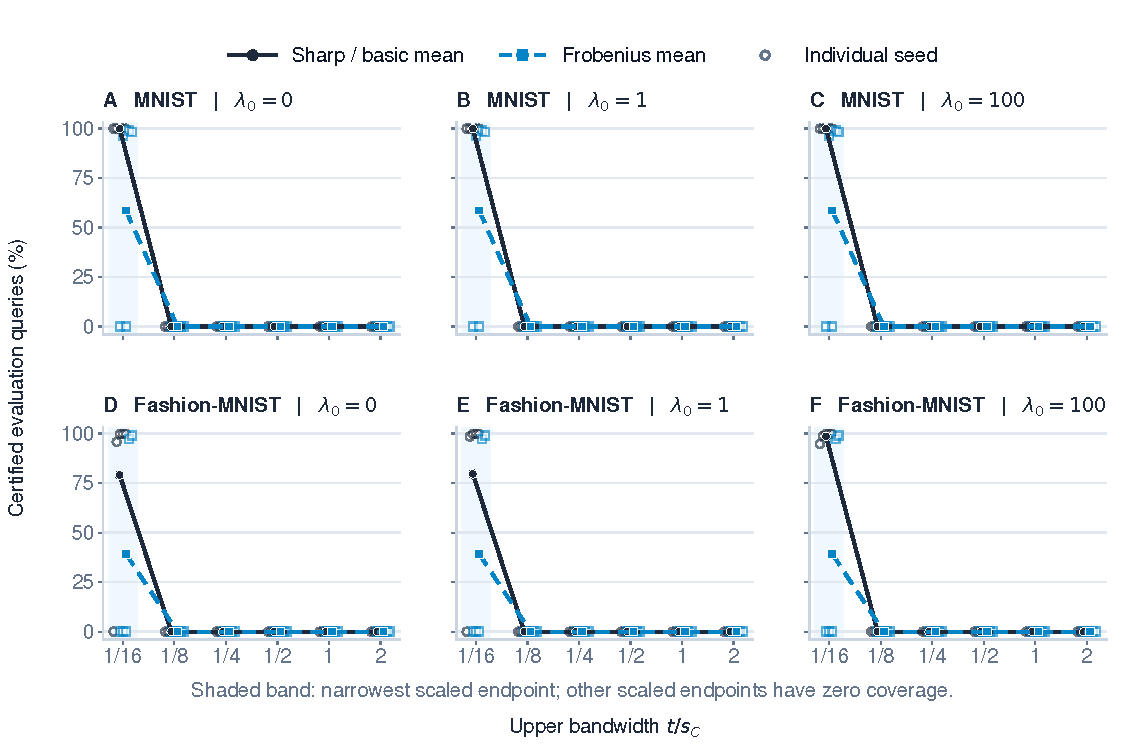
\includegraphics[width=\textwidth]{Figure_03_Certificate_Coverage.pdf}
\caption{Coverage of continuous parameter-region certificates at $K=100$. Columns correspond to penalty floors $\lambda_0=0,1,100$ and rows to MNIST and Fashion-MNIST. Navy shows the common sharp/basic mean and azure shows the Frobenius mean across five seeds; hollow markers show all individual seed percentages with small horizontal offsets. Sharp and basic certificate masks are identical. Each certified query satisfies the condition for every $0<\sigma\leq t$ and finite $\lambda\geq\lambda_0$. All six declared scaled endpoints are shown, with zero coverage at the displayed endpoints beyond $s_C/16$; the separate absolute endpoint $t=1$ also has zero coverage in every condition. Each seed uses the same 4,027 MNIST reserve images or 10,000 Fashion-MNIST test images. Values are taken directly from the archived per-seed analysis records; $s_C$ is defined in Eq.~\eqref{eq:scale}.}
\label{fig:coverage}
\end{figure}

\begin{table}[!htbp]
\centering\small
\caption{Certified coverage at $t=s_C/16$, reported as mean percentage $\pm$ sample standard deviation in percentage points across all five seeds. Sharp and basic have identical masks. The last column reports the number of zero-coverage seeds for the sharp and Frobenius methods, respectively. All methods have zero coverage at every other endpoint of the original grid.}
\label{tab:coverage}
\begin{tabular}{@{}lrrccc@{}}
\toprule
Dataset & $K$ & $\lambda_0$ & Sharp / basic (\%) & Frobenius (\%) & Zero seeds \\
\midrule
MNIST & 50 & 0 & $99.94\pm0.04$ & $78.29\pm43.79$ & 0 / 1 \\
 & 50 & 1 & $99.94\pm0.04$ & $78.29\pm43.79$ & 0 / 1 \\
 & 50 & 100 & $99.94\pm0.04$ & $78.29\pm43.79$ & 0 / 1 \\
 & 100 & 0 & $99.91\pm0.06$ & $58.68\pm53.57$ & 0 / 2 \\
 & 100 & 1 & $99.91\pm0.06$ & $58.68\pm53.57$ & 0 / 2 \\
 & 100 & 100 & $99.91\pm0.06$ & $58.68\pm53.57$ & 0 / 2 \\
 & 200 & 0 & $99.86\pm0.03$ & $0.00\pm0.00$ & 0 / 5 \\
 & 200 & 1 & $99.86\pm0.03$ & $0.00\pm0.00$ & 0 / 5 \\
 & 200 & 100 & $99.87\pm0.03$ & $0.00\pm0.00$ & 0 / 5 \\
\addlinespace
Fashion-MNIST & 50 & 0 & $99.33\pm1.35$ & $58.93\pm53.83$ & 0 / 2 \\
 & 50 & 1 & $99.71\pm0.48$ & $58.93\pm53.83$ & 0 / 2 \\
 & 50 & 100 & $99.77\pm0.35$ & $58.93\pm53.83$ & 0 / 2 \\
 & 100 & 0 & $79.09\pm44.25$ & $39.31\pm53.83$ & 1 / 3 \\
 & 100 & 1 & $79.63\pm44.52$ & $39.31\pm53.83$ & 1 / 3 \\
 & 100 & 100 & $98.66\pm2.22$ & $39.31\pm53.83$ & 0 / 3 \\
 & 200 & 0 & $79.06\pm44.23$ & $36.77\pm50.52$ & 1 / 3 \\
 & 200 & 1 & $79.54\pm44.47$ & $36.79\pm50.54$ & 1 / 3 \\
 & 200 & 100 & $98.54\pm2.26$ & $36.80\pm50.55$ & 0 / 3 \\
\bottomrule
\end{tabular}
\end{table}

At $K=100$, MNIST coverage is $99.91\pm0.06\%$ for each penalty floor. Fashion-MNIST coverage rises from $79.09\pm44.25\%$ at floor zero to $98.66\pm2.22\%$ at floor 100. The large dispersion at the lower floor includes one seed with zero coverage; all five seeds have positive coverage at floor 100. The same zero-seed pattern occurs for Fashion-MNIST at $K=200$. At $K=50$, both datasets have positive class-wise coverage in every seed and floor. These outcomes retain the seed realizations that account for the widest variation in Table~\ref{tab:coverage}.

The sharp and basic methods produce identical certification masks for every query in every region of the original grid. Their shared total is 587,703 certified query-region cases among 4,418,505 evaluated cases. The Frobenius method certifies a subset in every condition and certifies 285,286 cases in total. At $K=100$, its narrow-endpoint mean coverage is $58.68\%$ for MNIST and $39.31\%$ for Fashion-MNIST at each floor. At $K=200$, it certifies no MNIST query, whereas the class-wise conditions cover at least $99.86\%$ on average. Thus the experiment shows a coverage gain from preserving class-wise overlap information and zero realized coverage gain from the sharp envelope over the basic class-wise bound.

\subsection{Observed agreement and class accuracy}
The readout frequently agrees with the nearest-prototype label at endpoints whose regions receive zero certified coverage. At the absolute endpoint $t=1$, $K=100$, and $\lambda=0$, mean agreement is $97.82\%$ on MNIST and $98.27\%$ on Fashion-MNIST, while all certificate masks are empty. At the scaled endpoint $t=s_C/16$, agreement is $99.94\%$ and $99.91\%$, respectively. Figure~\ref{fig:agreement} shows these fitted-label relationships for the complete scaled-width grid, with accuracy displayed separately.

\begin{figure}[!htbp]
\centering
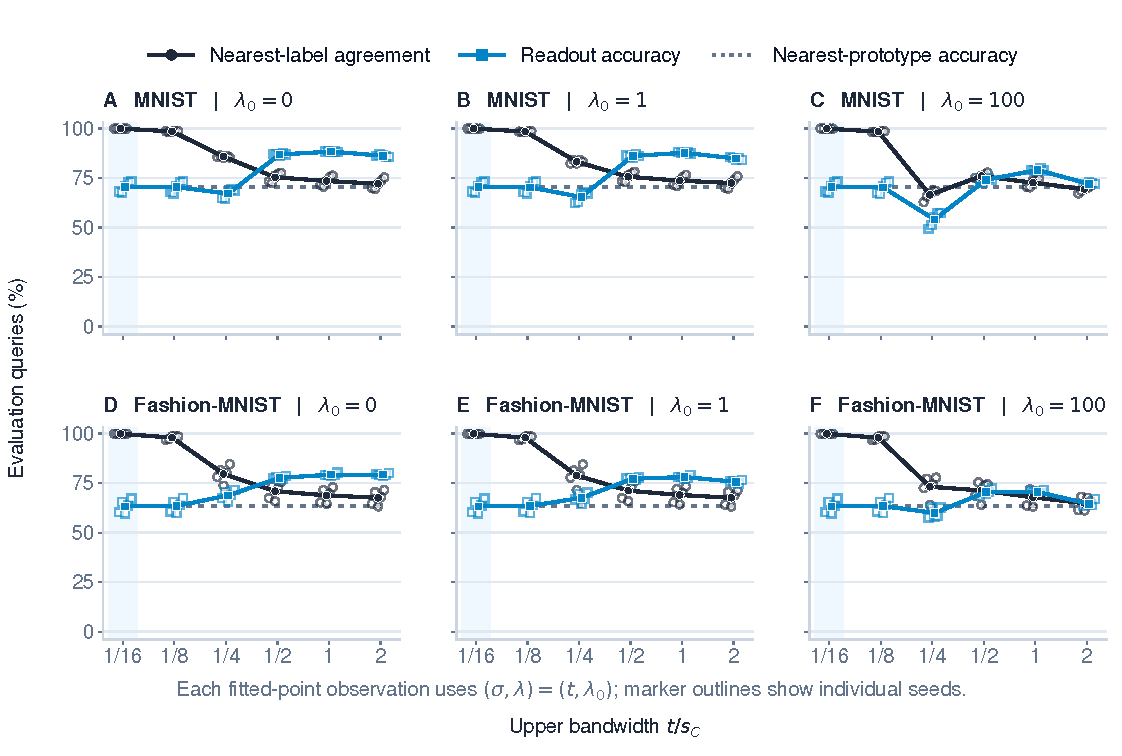
\includegraphics[width=\textwidth]{Figure_04_Agreement_Accuracy.pdf}
\caption{Fitted-point nearest-prototype agreement and class accuracy at $K=100$. Each endpoint fit uses $(\sigma,\lambda)=(t,\lambda_0)$. Navy curves report agreement between fitted-readout and nearest-prototype labels; azure curves report fitted-readout accuracy against held-out dataset labels; gray dotted lines report nearest-prototype accuracy. Lines join exact five-seed means from the archived analysis records; hollow markers show all individual seed outcomes for the two fitted-readout measures, with small horizontal offsets. All six scaled widths and all three penalty floors are included. Each seed uses the same 4,027 MNIST reserve images or 10,000 Fashion-MNIST test images. The gray baseline is constant because prototypes are fixed. These endpoint observations measure fitted labels; Fig.~\ref{fig:coverage} reports continuous-region certificate coverage.}
\label{fig:agreement}
\end{figure}

For $K=100$ and zero penalty, mean readout accuracy changes from $70.55\pm2.57\%$ at $s_C/16$ to $88.31\pm0.19\%$ at $s_C$ on MNIST. The corresponding Fashion-MNIST values are $63.30\pm3.22\%$ and $79.29\pm0.64\%$. Nearest-prototype accuracy remains $70.52\pm2.58\%$ and $63.29\pm3.23\%$ because the prototypes are fixed. At $s_C$, readout agreement with those prototype labels is $73.49\pm2.42\%$ on MNIST and $68.82\pm3.74\%$ on Fashion-MNIST. The broader model therefore has higher observed class accuracy in this comparison and a smaller fraction of decisions equal to the nearest-prototype label.

\subsection{Numerical verification}
All 5,289,327 finite-probe comparisons associated with regions certified by the sharp method agree with their nearest-prototype labels. Counting method-tagged checks for all three conditions gives 13,146,228 comparisons with zero violations. Deduplicating overlapping regions and methods within each dataset--seed--budget group yields 3,585,477 query-parameter checks, again with zero violations. These denominators describe repeated checks on the archived image queries. An independent reconstruction reproduced all 18 rows of Table~\ref{tab:coverage}, all 630 endpoint records, and all 1,890 certificate records. It rebuilt every certificate mask from the original image geometry and reconstructed 20,198,880 prediction labels from the stored readout weights with zero mismatches. A fresh execution of the complete frozen training pipeline reproduced all scientific arrays and all endpoint and certificate CSV measurements exactly.

Every selected prototype image is distinct within its group, and all 480 factorized feature matrices have full numerical column rank under the declared SVD cutoff. The 480 factorizations support 2,880 fitted readouts. The smallest certified raw margin is $1.47\times10^{-5}$, and the smallest certified margin-to-guard ratio is 51,145.07. All 71 frozen result-file hashes and all 30 prediction-freeze receipts were verified. The complete computational run, including prediction generation and scoring, took 123.20\,s. These checks connect the reported coverage to the frozen implementation and its archived predictions.
